Los Objetivos de Desarrollo Sostenible (\textit{ODS}), establecidos por las Naciones Unidas, constituyen un marco global que busca abordar los grandes desafíos sociales, económicos y medioambientales que enfrenta la humanidad. La investigación y el desarrollo tecnológico, especialmente en campos como la inteligencia artificial y el aprendizaje automático, pueden desempeñar un papel clave en la consecución de estos objetivos. Se definen de acuerdo al diagrama de la Figura 1:

\begin{figure}[H]
    {\begin{center}
    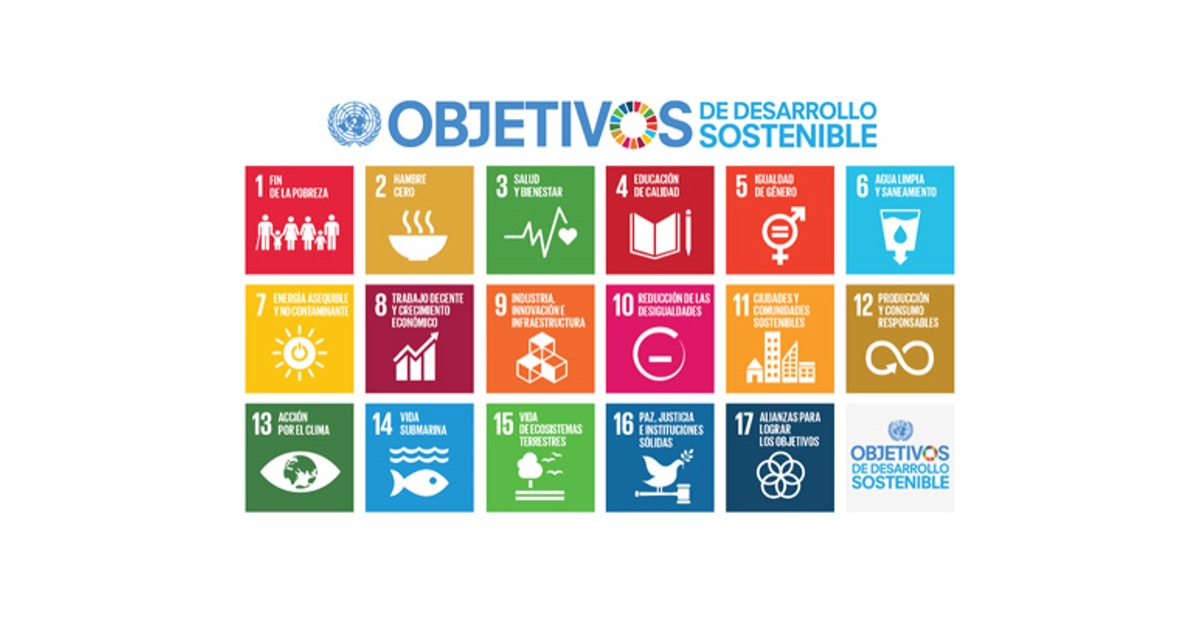
\includegraphics[width=0.7\textwidth]{commons/ODS.jpg}
    \caption{Objetivos de desarrollo sostenible}
    \label{fig:ODS}
    \end{center}}
\end{figure}

Este proyecto, centrado en el desarrollo y entrenamiento de modelos de aprendizaje automático con un objetivo concreto, siendo este la identificación y separación de elementos en una obra musical, se alinea con varios de los Objetivos de Desarrollo Sostenible establecidos por las Naciones Unidas. A continuación, se ponen en detalle los objetivos más relevantes con los que este proyecto presenta simpatía y se comenta la aportación de este a cada uno de ellos.

\section{ODS 4: Educación de calidad}
Este \textit{ODS} tiene como objetivo garantizar una educación inclusiva, equitativa y de calidad y promover oportunidades de aprendizaje durante toda la vida para todos.

El sistema presentado en este proyecto promueve oportunidades de aprendizaje para todos, identificando las funcionalidades más importantes de un modelo de aprendizaje automático , ilustrando las aplicaciones de estos en un ejemplo del mundo real , como puede ser la identificación de elementos en una obra musical y finalmente presentándolas al usuario de forma interactiva y transversal , con explicaciones por parámetro y método que permiten tanto a usuarios experimentados como a primerizos la interacción e introducción a esta tecnología que está cada día más presente en nuestras vidas.

\section{ODS 3: Salud y bienestar}
Este \textit{ODS} busca garantizar una vida sana y promover el bienestar para todos en todas las edades.

Si bien es sabido que el baile ( y el disfrute de la música ) es una actividad que , como ya se ha demostrado científicamente por multitud de estudios, promueve una mejora de la salud física  y emocional del individuo, la separación de fuentes de una obra es ampliamente utilizada para estos propósitos, bien por \textit{DJs} , \textit{Beatmakers} o \textit{Samplers} mediante diferentes técnicas dentro de estos ámbitos. Si bien esto se hacía antiguamente con métodos más rudimentarios , la introducción de la inteligencia artificial y en concreto de las redes neuronales artificiales como herramienta en este tipo de métodos , facilita y mejora el proceso , lo que deriva en el resultado de una mejor herramienta para el artista y por ende en disfrute para el público de este.

Además, este tipo de herramientas son ampliamente utilizadas para la práctica \textit{amateur} de instrumentos musicales , bien para obtener la pista musical de la guitarra en una canción y poder replicarla de oído en casa con tu propio instrumento , o bien para obtener la pista vocal y acompañarla con tu propia partitura.

Estas posibilidades que nos da la herramienta contribuyen lateralmente al bienestar emocional, abriendo bien un abanico de posibilidades creativas en casa o bien un abanico de mejoras en la metodología artística de los ``artesanos'' de estas disciplinas.